%%
%% Learning from AI-Assisted Developer Workflows
%% Vision Paper - ACM sigconf format
%%
\documentclass[sigconf]{acmart}

\AtBeginDocument{%
  \providecommand\BibTeX{{Bib\TeX}}}

\setcopyright{acmlicensed}
\copyrightyear{2025}
\acmYear{2025}
\acmDOI{XXXXXXX.XXXXXXX}

\acmConference[Conference acronym 'XX]{Make sure to enter the correct
  conference title from your rights confirmation email}{Month DD--DD,
  2025}{City, Country}
\acmISBN{978-1-4503-XXXX-X/2025/XX}

\usepackage{tikz}
\usetikzlibrary{arrows.meta, positioning}
\usepackage[table]{xcolor}
\usepackage{tabularx}
\usepackage{array}

\begin{document}

\title{Tracing Your Steps: Learning from AI-Assisted Developer Workflows}

\author{Hamidah Oderinwale}
\email{hamidah.oderinwale@mail.mcgill.ca}
\affiliation{%
  \institution{McGill University}
  \city{Montreal}
  \state{Quebec}
  \country{Canada}
}

\renewcommand{\shortauthors}{Oderinwale}

\begin{abstract}
AI-augmented programming has become ubiquitous, yet three fundamental gaps remain: (1) we lack principled identification of what signals in real workflows are learnable and valuable, (2) we do not understand how those signals should evaluate and improve code agents, and (3) we have no representation layer that makes raw IDE telemetry comparable, shareable, and governable at scale. We argue that AI evaluation must move from static benchmarks to \emph{in-vivo} measurement of real developer--agent workflows. We propose representation dimensions that transform raw logs into structured abstractions---files, motifs, and context flows---enabling \emph{evals in the wild}. These representations make it possible to measure, compare, and optimize how software is produced, not just what code is output. We outline how this substrate supports personalization, collective learning, and governance of AI-assisted software engineering, and identify key research questions that must be addressed to realize this vision.
\end{abstract}

\begin{CCSXML}
<ccs2012>
 <concept>
  <concept_id>10011007.10011006.10011008</concept_id>
  <concept_desc>Software and its engineering~General programming languages</concept_desc>
  <concept_significance>500</concept_significance>
 </concept>
 <concept>
  <concept_id>10010147.10010257</concept_id>
  <concept_desc>Computing methodologies~Machine learning</concept_desc>
  <concept_significance>500</concept_significance>
 </concept>
 <concept>
  <concept_id>10011007.10011006.10011066</concept_id>
  <concept_desc>Software and its engineering~Software development techniques</concept_desc>
  <concept_significance>300</concept_significance>
 </concept>
</ccs2012>
\end{CCSXML}

\ccsdesc[500]{Software and its engineering~General programming languages}
\ccsdesc[500]{Computing methodologies~Machine learning}
\ccsdesc[300]{Software and its engineering~Software development techniques}

\keywords{AI-assisted development, code generation, workflow analysis, developer telemetry, program synthesis, evaluation}

\maketitle

\section{Introduction}

\textbf{Developers produce systems faster than they understand them.} As programming becomes declarative---developers writing prompts that instruct agents to generate code---a new interpretability crisis emerges. Repositories provide little insight into how systems were constructed, how they evolved, or why particular decisions were made.

\textbf{Development is iterative, but evaluation is not.} AI-assisted development is interactive, iterative, and feedback-driven: navigation, experimentation, testing, repair. Yet evaluations treat development as single-shot. Benchmarks like HumanEval~\cite{chen2021evaluating}, MBPP~\cite{austin2021program}, and SWE-bench~\cite{jimenez2024swebenchlanguagemodelsresolve} measure performance on isolated puzzles, assuming well-defined tasks and enumerable success criteria. Empirical studies of developer--model interactions~\cite{barke2023grounded} reveal complex workflows involving prompt refinement, code review, and selective acceptance---patterns invisible to static benchmarks but central to understanding AI-assisted development.

\textbf{The central bottleneck is representation.} We must move from evaluating \emph{code} to evaluating \emph{workflows}. This requires a representation layer that makes real-world developer activity measurable, comparable, and steerable.

\textbf{This paper's contribution.} We articulate a vision for workflow-based evaluation of AI-assisted development. We propose representation dimensions that transform raw telemetry into structured abstractions, outline how these representations enable new forms of evaluation, personalization, and governance, and identify the research questions that must be addressed to realize this vision.

\section{The Case for Workflow Evaluation}

\textbf{Repositories capture snapshots, not process.} Existing benchmarks measure whether a model produces a correct solution for a predefined task. Version control captures only a thin slice: published snapshots, stripped of exploratory and corrective work.

\textbf{Observing real workflows informs benchmark design.} Understanding what developers actually do with AI---which tasks they attempt, how they iterate, where they struggle---reveals gaps in static benchmarks. If real workflows show developers frequently refactor multi-file modules, benchmarks should include refactoring tasks. In-vivo measurement informs benchmark design, making evaluations more realistic.

\textbf{To improve agents, we must evaluate them as developers.} This means measuring how they search, refactor, test, recover from errors, manage context, and coordinate across files. These behaviors are present in live telemetry but invisible in repositories. We therefore propose \emph{evals in the wild}: evaluations on real developer--agent interactions.

\textbf{Observability depends on the interface.} Cursor captures IDE-integrated workflows, Claude Code operates via CLI, developers using chatbots may copy code into traditional IDEs---each form factor differs in autonomy and interaction patterns. The representation framework generalizes by abstracting tool-specific details into common workflow patterns.

\textbf{Prior work enables component analysis but misses multi-modal workflows.} Clio~\cite{clio2024} demonstrated that clustering conversations reveals usage patterns while preserving privacy. OverCode~\cite{glassman2015overcode} showed that canonicalizing student solutions enables comparison across thousands of programs. Seymour~\cite{kasibatla2017seymour} demonstrated real-time visualization of program execution; our vision extends this to production-scale AI-assisted development, where the ``program'' visualized is the developer--agent interaction itself. Recent work on discovering latent structure in LLM interactions~\cite{huang2025values} shows that meaningful categories emerge bottom-up from embeddings and clustering. Platforms can use information design to solve incentive problems~\cite{haghtalab2024platforms}. However, these approaches face limitations: Clio clusters prompts but misses code changes, files navigated, tests run, and reverts. Clustering for text conversations does not capture multi-modal, temporally-structured development workflows.

Microsoft's SPACE framework formalized productivity as multi-dimensional~\cite{forsgren2021space}. An alternative derives evaluation signals from real traces~\cite{donyehiya2024future}, identifying model-task pairs where users frequently revert changes.

\section{The Companion System}

\textbf{Fine-grained telemetry with negligible overhead.} We describe a companion system that captures development traces from Cursor. The system records five event classes: code changes, prompts, context snapshots, terminal commands, and conversations (Table~\ref{tab:companion}).

\begin{table}[t]
\centering
\caption{Companion system event types and captured fields.}
\label{tab:companion}
\small
\renewcommand{\arraystretch}{1.3}
\rowcolors{2}{gray!10}{white}
\begin{tabular}{>{\bfseries}l p{5.2cm}}
\toprule
\rowcolor{gray!25}
\textbf{Event Type} & \textbf{Fields Captured} \\
\midrule
Code change & file path, diff, lines added/removed, timestamp, session \\
Prompt & prompt text, response, model, context files, timestamp \\
Context snapshot & files in context, token counts, truncation status \\
Terminal command & command, working directory, exit code, duration \\
Conversation & conversation ID, prompt sequence, session linkage \\
\bottomrule
\end{tabular}
\end{table}

Raw traces are stored locally by default. Developers choose which abstraction levels to share, maintaining control over data and privacy. The system exposes representations through an API, enabling organizations to query workflow patterns without direct access to raw telemetry.

\section{From Traces to Representations}

\textbf{Raw telemetry must be decomposed into structured objects.} Raw telemetry is too noisy, large, and siloed to study directly. We propose representation dimensions that decompose workflows into structured objects: files (what exists and changes), motifs (recurring procedural subsequences), and context flows (how attention propagates through a workspace).

\textbf{The choice of representation shapes what can be observed.} The choice fundamentally shapes what can be observed, measured, and learned~\cite{representation2024}. Motifs capture procedural patterns, semantic edits capture structural intent, module graphs capture architectural coupling. Each dimension functions as a lens that makes certain signals visible while compressing others. Following principles for multiple views in information visualization~\cite{wang2000guidelines}, the framework provides complementary perspectives.

\textbf{Events are the atomic unit of workflow analysis.} Workflows decompose into sequences of events---prompts, code changes, tests, navigation---each representing a discrete action. Events are observable, timestamped, and semantically meaningful: finer than keystrokes but coarser than full sessions.

\textbf{Intent-based segmentation aligns better with task semantics.} Traditional segmentation uses inactivity to signal task boundaries. AI-assisted development challenges this: a prompt may initiate a new task without time gaps. Intent-based segmentation (prompt-driven, semantic) aligns better with task semantics than temporal segmentation.

\textbf{Temporal structure encodes efficiency invisible to static analysis.} Code analysis focuses on static structure. Workflow analysis reveals temporal structure: edit order, change propagation, development rhythm. Temporality encodes efficiency: developers editing related files in quick succession may be more efficient than those scattering edits.

Rather than a strict hierarchy, these dimensions function like principal components: procedural patterns (motifs), structural intent (semantic edits), architectural coupling (module graph), API evolution (functions). Each preserves different signals while compressing noise.

\textbf{Grammar induction discovers recurring procedural structure.} We treat each trace as a sequence over a small alphabet of typed events: prompt, edit, test, error, navigation, commit. Sequential pattern mining (PrefixSpan) identifies frequent subsequences; grammar-based compression (Sequitur) introduces reusable rules when patterns repeat. The induced rules are \emph{motifs}: compact procedural building blocks like debug loops, refactoring bursts, or configuration cascades. Library learning discovers reusable abstractions from structured data~\cite{wang2020library,bowers2023topdown}; prior work shows humans naturally converge on shared procedural abstractions~\cite{mccarthy2021learning}; motifs formalize this for software development.

\textbf{Motifs are learnable procedural subroutines.} Motifs are discovered through a two-stage process: statistical sequence mining extracts recurring patterns; intent categories emerge bottom-up through embedding and clustering~\cite{huang2025values}. Event descriptions are embedded using sentence transformers and clustered with HDBSCAN to discover natural groupings. This discovers fine-grained intents like ``major refactoring with character changes'' rather than predefined categories like DEBUG.

Privacy can be configured at deployment time. Identifiers can be canonicalized: the same pipeline produces either \texttt{src/auth/login.tsx} or \texttt{F\_a3b2c1d4} depending on policy. Intent categories can be prescribed (DEBUG, REFACTOR, TEST) for fast, interpretable analysis, or discovered bottom-up for richer coverage. Both are policy levers, not architectural constraints.

\textbf{Organizing discovered intents: flat versus hierarchical taxonomies.} How should intent categories be discovered and organized? This question is fundamental because different organizational structures enable different types of analysis. We explored both flat and hierarchical approaches, finding that the choice of taxonomy structure shapes what patterns become visible.

\textbf{Flat clustering discovers fine-grained categories.} We first explored flat clustering: event descriptions are embedded and clustered with HDBSCAN to produce a single-level taxonomy. This discovers fine-grained categories like ``major refactoring with character changes'' without imposing hierarchical structure. Flat taxonomies are interpretable and sufficient for many comparison tasks, but they may miss multi-granularity relationships. A ``refactoring'' category might contain both ``structural refactoring'' and ``naming refactoring'' sub-patterns that could be distinguished at finer granularity.

\textbf{Hierarchical clustering enables multi-level analysis.} Clustering at different levels is an interesting research question because it enables multi-granularity analysis: the same workflow can be analyzed at different abstraction levels depending on the question. We implemented two hierarchical strategies: (1) \emph{Agglomerative hierarchical clustering} builds bottom-up trees by iteratively merging similar clusters, producing multi-level taxonomies where level 0 represents individual events, level 1 represents fine-grained sub-clusters (e.g., ``fix null pointer''), level 2 represents medium-grained clusters (e.g., ``error handling''), and level 3 represents coarse-grained super-clusters (e.g., ``debugging''). (2) \emph{Recursive clustering} (inspired by Clio~\cite{clio2024}) uses multi-level summarization: events are first clustered into sub-clusters, then sub-clusters are recursively clustered into higher-level categories. This recursive process aligns taxonomies with human understanding while preserving bottom-up discovery.

\textbf{The level of clustering shapes what becomes visible.} Hierarchical taxonomies reveal different patterns than flat ones. At fine granularity, we see specific intents like ``fixing off-by-one errors''; at coarse granularity, we see broader patterns like ``debugging workflows.'' This multi-level structure enables targeted analysis: researchers can query workflows at the appropriate abstraction level for their question. However, hierarchical taxonomies introduce complexity: they require choosing the number of levels, determining cluster boundaries, and interpreting multi-level relationships. Our comparison of flat versus hierarchical approaches reveals tradeoffs: flat taxonomies are simpler and faster to compute, while hierarchical taxonomies capture richer structure but require more careful interpretation.

\textbf{Unexplored directions: procedure-aware and representation-level clustering.} Several directions remain unexplored. \emph{Hierarchical dimensionality reduction} could first project embeddings into lower-dimensional spaces that capture coarse-grained structure, then discover fine-grained categories within each subspace. \emph{Hierarchical annotation} could combine prescribed top-level domains (DEBUG, REFACTOR, FEATURE) with emergent sub-categories discovered bottom-up within each domain, enabling both consistency and expressiveness. \emph{Procedure-aware clustering}, which accounts for temporal sequence, edit dependencies, and workflow structure, is largely unexplored: current approaches cluster event descriptions independently, but future work could cluster motifs (sequences) directly, incorporate temporal proximity, or use graph-based clustering over workflow dependency structures. This would align categories with procedural patterns rather than just semantic similarity of individual events. \emph{Representation-level abstraction} could cluster at different rungs of the representation hierarchy: clustering at the motif level might reveal different patterns than clustering at the semantic edit level, enabling targeted discovery of procedural versus structural intent patterns.

\textbf{Privacy is a multi-dimensional guarantee.} Privacy has three dimensions: \emph{reconstructability} (can the original trace be recovered?), \emph{identifiability} (can the source developer be identified?), and \emph{information leakage} (what sensitive data persists?). Different representation levels provide different guarantees: tokens canonicalize identifiers but preserve syntax; semantic edits preserve intent but discard code; motifs preserve procedural patterns but discard code and paths.

\begin{table*}[t]
\centering
\caption{Representation dimensions: each level captures a distinct aspect of developer workspaces with different privacy-compression tradeoffs. Compression ratios are illustrative targets.}
\label{tab:rung_hierarchy}
\small
\renewcommand{\arraystretch}{1.2}
\rowcolors{2}{gray!10}{white}
\begin{tabularx}{\textwidth}{>{\bfseries}l >{\raggedright\arraybackslash}X >{\raggedright\arraybackslash}X >{\raggedright\arraybackslash}X >{\raggedright\arraybackslash}X}
\toprule
\rowcolor{gray!25}
\textbf{Level} & \textbf{Captures} & \textbf{Preserves} & \textbf{Abstracts Away} & \textbf{Primary Use} \\
\midrule
Raw & Code, prompts, metadata & Full semantic detail & --- & Session debugging \\
Tokens & Canonicalized token types & Syntax structure & Identifiers, literals & Code similarity \\
Semantic Edits & Operation $\rightarrow$ target pairs & Edit intent & Implementation details & Workflow pattern detection \\
Functions & Function-level changes & Which functions changed & Statement-level detail & API evolution tracking \\
Module Graph & File relationships, co-editing & Coupling patterns & Intra-file changes & Dependency analysis \\
Motifs & Procedural patterns & Workflow strategies & Surface variation & Strategy comparison \\
\bottomrule
\end{tabularx}
\end{table*}

We characterize representations along dimensions: \emph{length} (terms per trace) measures granularity; \emph{vocabulary} (unique terms) measures semantic richness; \emph{uniqueness} (percentage distinct) proxies for identifiability; \emph{entropy} measures expressiveness. The $\epsilon$-gap between intra-trace similarity (fidelity) and inter-trace similarity (blending) quantifies identifiability.

\textbf{Representations are configurable by goal.} Learning may require high expressiveness (semantic edits); privacy may require low reconstructability (motifs); analytics may tolerate higher identifiability if leakage is bounded. The representation layer is a configurable system where level selection, canonicalization policies, and intent extraction methods are chosen based on the goal.

\textbf{Procedural patterns distinguish workflows that produce similar outputs.} Consider two developers. One refactors: modifies multiple functions, deletes unused code, updates imports. Another adds a feature: creates new files, adds functions, updates configuration, writes tests. Both involve code changes, but procedural patterns differ: refactoring shows rapid file switching and deletions; feature addition shows sequential creation and expansion.

Traditional approaches use normative taxonomies: predefined categories (DEBUG, REFACTOR, FEATURE) that impose structure. However, development exhibits intricate facets that resist reduction to fixed categories. A normative approach risks oversimplification: both workflows might be labeled FEATURE, obscuring procedural differences.

Emergent intent discovery addresses this by discovering natural groupings bottom-up, following~\cite{huang2025values}. Event descriptions are embedded and clustered across thousands of sessions, revealing categories like ``Major Refactoring Cluster,'' ``Large addition,'' ``Configuration,'' ``Test-related,'' and ``Documentation'' that emerge from data rather than being prescribed. Sequence mining extracts transitions like \texttt{EV\_a13f92} $\rightarrow$ \texttt{EV\_10c99d} (file switches) and structural patterns like \texttt{HOTSPOT\_8} (many edits in one file), assigned to discovered intent categories. Fine-grained categories capture procedural differences invisible to coarse taxonomies.

\textbf{Structural patterns transfer where surface tokens do not.} Two developers may produce similar outputs yet follow different paths. Motifs and context flows reveal how they structured work and responded to feedback. Structural patterns generalize better than raw content~\cite{yun2023emergence}. Discovered intent clusters work across Python, TypeScript, and Java; token sequences are language-specific. Intent labels attach semantic meaning to structural patterns, turning opaque sequences into readable strategies. This framework mirrors abstract interpretation~\cite{cousot1977abstract}, where each dimension defines an abstract domain trading precision for preserved structure.

\begin{figure}[t]
\centering
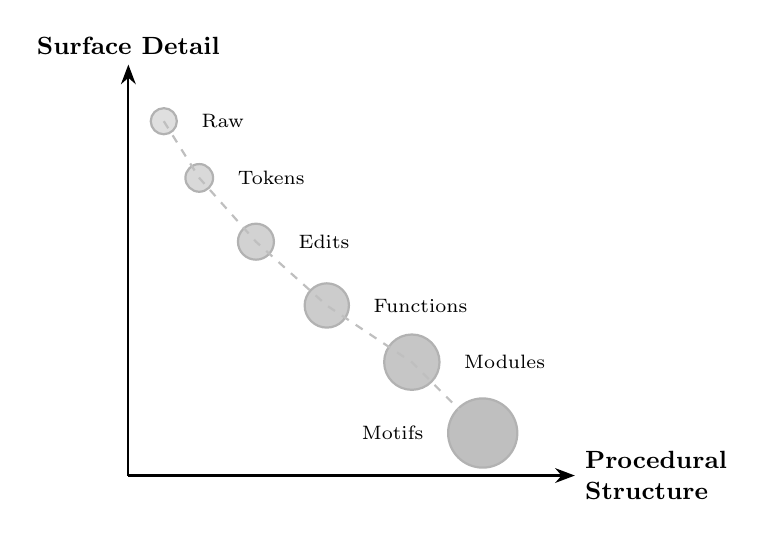
\begin{tikzpicture}[
    scale=0.9,
    axis/.style={-{Stealth[length=2.5mm]}, thick},
    rung/.style={circle, draw=black!30, thick},
    runglabel/.style={font=\scriptsize},
    dimlabel/.style={font=\small\bfseries}
]

\draw[axis] (0,0) -- (0,5.8) node[above, dimlabel, align=center] {Surface Detail};
\draw[axis] (0,0) -- (6.3,0) node[right, dimlabel, align=left] {Procedural\\Structure};

\node[rung, fill=gray!25, minimum size=8pt] (raw) at (0.5, 5.0) {};
\node[runglabel, right=5pt] at (raw.east) {Raw};

\node[rung, fill=gray!30, minimum size=10pt] (tokens) at (1.0, 4.2) {};
\node[runglabel, right=5pt] at (tokens.east) {Tokens};

\node[rung, fill=gray!35, minimum size=13pt] (edits) at (1.8, 3.3) {};
\node[runglabel, right=5pt] at (edits.east) {Edits};

\node[rung, fill=gray!40, minimum size=16pt] (functions) at (2.8, 2.4) {};
\node[runglabel, right=5pt] at (functions.east) {Functions};

\node[rung, fill=gray!45, minimum size=20pt] (modules) at (4.0, 1.6) {};
\node[runglabel, right=5pt] at (modules.east) {Modules};

\node[rung, fill=gray!50, minimum size=25pt] (motifs) at (5.0, 0.6) {};
\node[runglabel, left=5pt] at (motifs.west) {Motifs};

\draw[dashed, gray!50, line width=0.8pt] 
    (raw.center) -- (tokens.center) -- (edits.center) -- 
    (functions.center) -- (modules.center) -- (motifs.center);

\end{tikzpicture}
\Description[Representation dimensions]{Six representation levels positioned along axes of Surface Detail and Procedural Structure.}
\caption{Representation dimensions. Each level captures a different aspect of developer workspaces. Higher levels preserve procedural structure while compressing surface detail.}
\label{fig:rung_dimensions}
\end{figure}

\section{Enabling Evals in the Wild}

\textbf{Representations make workflows measurable and comparable.} Representations turn workflows into objects that can be measured, compared, and optimized. \emph{Intra-trace similarity} measures how well a representation preserves information within a trace; \emph{inter-trace similarity} measures how similar traces become after abstraction. The $\varepsilon$-gap quantifies identifiability: a large gap means traces remain distinguishable; a small gap means traces blend together.

Higher levels reduce identifiability: motifs achieve higher inter-trace similarity (blending), tokens achieve lower (distinguishable). The representation dimensions enable searching across workspaces for workflows satisfying specific properties: refactoring patterns (motif dimension), API evolution (function dimension), architectural changes (module graph).

\textbf{Privacy, expressiveness, and utility are separate dimensions.} Abstraction is usually framed as privacy versus utility. But these are separate dimensions. Higher abstraction can \emph{increase} utility: raw traces are noisy, motifs expose transferable procedure. A debug loop motif works across Python, TypeScript, and Java; raw token sequences do not. Organizations select levels based on which privacy dimension matters: compliance may require low reconstructability (motifs); research may tolerate higher identifiability if leakage is bounded.

\textbf{Evaluation becomes comparison of workflows, not final code.} Two models are evaluated by comparing how they work: edit patterns, context use, error recovery, codebase navigation. Models can be matched to tasks based on procedural fit rather than benchmark scores alone.

\textbf{Compression reduces cognitive load.} A developer reviewing thousands of sessions cannot inspect raw traces~\cite{miller1956magical,gero2024sensemaking}. Higher levels achieve compression; at the motif level, developers see workflow patterns rather than keystrokes.

\textbf{Each level optimizes for different analysis and privacy goals.} Tokens support code completion evaluation. Semantic edits support refactoring detection. Functions support API evolution. Module graph supports architectural drift. Motifs support workflow classification and governance. Context retrieval---finding relevant files for a prompt---trades retrieval performance for privacy across levels.

\textbf{Probes measure which signals survive abstraction.} Rather than ablating model components, we ablate representational access and measure performance degradation. Train linear classifiers on representations to measure predictive signal content. If a probe achieves high accuracy on motifs but low on tokens, procedural structure survives abstraction while syntactic detail does not.

\textbf{Procedural search transforms development history into a knowledge base.} The representation dimensions enable searching across workspaces for workflows satisfying specific properties. This enables \emph{procedural search}: developers discovering how others solved similar problems by querying workflow patterns (``test-driven refactoring workflows'') or intent categories (``debugging sessions that led to fixes'') rather than code content. This connects to procedural knowledge libraries~\cite{oderinwale2025proceduralknowledgelibrariesexecutable}: workflow representations encode not just what code exists but how it was produced.

\section{Steering Software Engineering}

\textbf{Workflows become steerable once represented.} Objectives can be defined over processes: minimizing context churn, encouraging test-driven loops, limiting cascade edits from fragile files. These constraints act as regulatory pressures, shaping how agents and humans work together. This enables process governance: organizations specify how development should proceed, not just what code should look like.

\textbf{Closed-loop evaluation surfaces inefficiencies in real-time.} Representations extracted in real-time can surface inefficiencies: excessive revision cycles, fragile context selection, cascading edits from unstable files. These signals feed back into behavior. Agents can be constrained by workflow objectives, not just output correctness. Developers see which strategies succeed before committing to them. Evaluation becomes concurrent with development.

\textbf{Change propagation reveals leverage points.} Modifying file $A$ triggers changes to $B$, $C$, $D$, forming directed propagation graphs. These cascades reveal architectural leverage: some files trigger many downstream changes. Understanding propagation guides engineering priorities.

\textbf{Emergent intents guide research priorities.} Static benchmarks measure output correctness but cannot identify which workflow patterns correlate with success. Emergent intent discovery reveals which procedural strategies succeed at fine granularity. Instead of ``How do we improve code generation?'' we ask ``Which intent patterns correlate with efficient task completion?'' Representations make these questions empirically tractable.

\section{The Vision: Crowdsourced Workflow Intelligence}

\textbf{High-level abstractions enable collective learning.} The long-term goal is a shared substrate for learning from real development while preserving privacy. High-level abstractions can be safely shared, enabling collective intelligence about effective development. Humans naturally converge on shared procedural abstractions~\cite{mccarthy2021learning}; developers and agents can build a common vocabulary through aggregated motif distributions. Platforms with information advantages can structure signals to steer agents toward efficient collaboration~\cite{haghtalab2024platforms}; the representation layer provides such an advantage.

\textbf{Workflow representations unlock evaluation, shared vocabulary, and collective learning.} Three capabilities become possible: (1) Evaluate code agents based on how they perform real software engineering across environments. (2) A shared language for analyzing and comparing workflows at scale. (3) Aggregate and learn from patterns while preserving privacy.

\textbf{Representations enable bidirectional alignment.} Developers orchestrate agents through declarative specifications, but current orchestration is blind: models are chosen by benchmark scores, not procedural fit. Representations enable bidirectional alignment: (1) \emph{Aligning AI to developer needs}---measuring how models work (motif distributions, error recovery, context strategies) enables matching models to tasks empirically. (2) \emph{Aligning developers to AI capabilities}---representations reveal which strategies succeed. Developers learn which strategies are effective while maintaining control.

\textbf{Motif-aware training rewards efficient procedures, not just correct outputs.} Current agent training asks: did it produce correct code? Motif-aware training adds: did it follow efficient procedures? This matters when agents must be interpretable or supervised---\emph{how} a problem is solved affects whether humans can understand, correct, or trust the process.

\section{Discussion}

\textbf{Implications for evaluation and learning.} This framework shows that learning from program traces in the wild is possible. Workflows exhibit network properties that provide vocabulary for understanding how development unfolds. Abstraction trades expressiveness for privacy in predictable ways: higher levels achieve compression while preserving structural patterns that generalize across languages. Different abstraction levels reveal different causal chains: motifs show pattern-to-task-type relationships, semantic edits show edit-sequence-to-workflow relationships, functions show pattern-to-code-organization relationships.

\textbf{Procedural structure may persist under compression.} Prior work has shown that sequence models develop abstract state representations even when intermediate observations are withheld~\cite{yun2023emergence}. Workflow abstractions may behave similarly: encoding task-relevant signals despite compressing surface detail. Probing offers a methodology to test this. If procedural structure persists at high compression while syntax does not, representations have learned to separate strategy from surface.

\textbf{Limitations and assumptions.} This framework makes several assumptions requiring validation. It assumes procedural patterns are learnable and transferable across contexts---that a debug loop in Python shares structure with one in TypeScript. It assumes abstraction preserves needed signals for downstream tasks. It assumes developers will share workflow data at some abstraction level, which depends on trust and privacy guarantees. It requires sufficient telemetry coverage---sparse or noisy traces may yield unreliable representations. It assumes workflow quality can be measured independently of task outcomes, which may not hold for exploratory or creative work.

\textbf{Open questions at the representation level.} What is the minimum abstraction that preserves a given class of patterns? How do emergent clusters evolve---do they stabilize, drift, or converge? Can we distinguish stable procedural preferences from situational responses?

\textbf{Open questions at the learning level.} Do motifs transfer across languages, teams, or domains? Do agent workflows converge toward common patterns? Can we learn procedural templates encoding engineering constraints independent of syntax?

\textbf{Open questions at the systems level.} Can we predict which files will be edited next based on current workflow patterns? Dynamic link prediction~\cite{kapoor2020dynamic} could enable proactive context loading. What protocols enable federated learning without centralizing traces? Can procedural profiles become portable?

\textbf{Open questions at the evaluation level.} What constitutes good workflow? How do we define quality when developers pursue diverse goals? Can workflow quality be measured independently of task outcomes?

\section{Conclusion}

We have argued that AI evaluation must move from static benchmarks to in-vivo measurement of real developer--agent workflows. We propose representation dimensions that transform raw logs into structured abstractions---files, motifs, context flows---enabling evals in the wild. These representations make it possible to measure, compare, and optimize how software is produced.

The core insight is that abstraction trades expressiveness for privacy in predictable ways: higher levels achieve compression while preserving structural patterns that generalize across languages. This creates a design space where level selection, canonicalization policies, and intent extraction methods are configured based on whether the goal is learning, privacy, analytics, or governance.

Representations make workflows measurable. Closed-loop evaluation makes them steerable. As AI-assisted development becomes ubiquitous, the ability to learn from real workflows---not just static artifacts---will determine whether we build systems that improve how software is made.

\bibliographystyle{ACM-Reference-Format}
\bibliography{main}

\end{document}
